\documentclass[11pt, a4paper]{article}

% ── Packages ──────────────────────────────────────────────────────────────────
\usepackage[margin=2.5cm]{geometry}
\usepackage{amsmath, amssymb}
\usepackage{booktabs}
\usepackage{multirow}
\usepackage{graphicx}
\usepackage{xcolor}
\usepackage{hyperref}
\usepackage{caption}
\usepackage{subcaption}
\usepackage{microtype}
\usepackage{natbib}
\usepackage{algorithm}
\usepackage{algpseudocode}
\usepackage{listings}
\usepackage{float}
\usepackage{enumitem}
\usepackage{parskip}

\hypersetup{
  colorlinks=true,
  linkcolor=blue!70!black,
  citecolor=green!50!black,
  urlcolor=blue!70!black
}

% ── Title ─────────────────────────────────────────────────────────────────────
\title{%
  \textbf{Replicating xRFM: Accurate, Scalable, and Interpretable\\
  Feature Learning Models for Tabular Data +bonus}\\[0.5em]
  \large COMP9417 Group Project
}

\author{
  Xueyao Jiang z5581908 \and
  Chang Yang z5569348 \and
  Binyue Peng z5705242 \and
  Jiayu Zhang z5649264 \and
  Zirun Zhang z5617187
}

\date{\today}

% ── Document ──────────────────────────────────────────────────────────────────
\begin{document}

\pagenumbering{gobble}
\maketitle
\tableofcontents
\newpage
\pagenumbering{arabic}
\setcounter{page}{1}

% ── Sections ──────────────────────────────────────────────────────────────────
% ── Section 1: Introduction ───────────────────────────────────────────────────
% Responsible: B (xRFM person)
% Placeholder — to be filled by B

\section{Introduction}

% TODO (B): Write introduction covering:
%   - Challenges of tabular data prediction
%   - Motivation: why xRFM over GBDTs?
%   - Core idea of xRFM (AGOP + tree structure)
%   - Overview of experiments (A provides 1-2 sentences on datasets)
%   - Structure of the report

\textit{[Placeholder: Introduction to be written by B. Covers tabular data challenges, xRFM motivation, experimental overview.]}

Tabular data constitutes one of the most pervasive forms of data in industry and science \citep{grinsztajn2022tree}.
Despite dramatic advances in deep learning for images and text, Gradient Boosted Decision Trees (GBDTs) such
as XGBoost \citep{chen2016xgboost} and LightGBM \citep{ke2017lightgbm} remain the dominant approach for tabular
prediction tasks. Recently, \citet{beaglehole2025xrfm} proposed \textit{xRFM}, a model that combines
feature-learning kernel machines with an adaptive binary tree structure, achieving state-of-the-art results
on the TALENT benchmark.

In this report, we replicate the core experiments of \citet{beaglehole2025xrfm}, evaluating xRFM
against three baseline models — XGBoost, LightGBM, and MLP — across five tabular datasets spanning
regression and binary classification tasks. We further analyse scalability and interpretability to
contextualise the strengths and limitations of xRFM in practice.

% Section 2: Methodology

\section{Methodology}

\subsection{xRFM: Algorithm and Theoretical Background}

xRFM is a tabular feature-learning model based on the Average Gradient Outer Product (AGOP)~\citep{beaglehole2025xrfm,radhakrishnan2024mechanism}. For a learned prediction function $f:\mathbb{R}^{d}\rightarrow\mathbb{R}$, the AGOP is defined as
\begin{equation}
    G_f=\mathbb{E}_{x}\!\left[\nabla f(x)\nabla f(x)^{\top}\right],
    \label{eq:agop}
\end{equation}
where $\nabla f(x)$ measures the sensitivity of the prediction to each input feature. Large diagonal values of $G_f$ indicate features that strongly affect the learned function. In this project, we use the diagonal AGOP setting because it is cheaper than storing the full $d\times d$ matrix and gives direct feature-level importance scores.

The key intuition is that AGOP provides a supervised view of feature relevance. PCA identifies high-variance input directions without using the target variable~\citep{pearson1901pca}; mutual information measures feature-target dependence mostly at the individual-feature level~\citep{kraskov2004estimating}; and permutation importance measures post-hoc test-performance degradation~\citep{fisher2019all}. By contrast, AGOP is derived from the gradients of the fitted model, so it reflects the directions that the prediction function actually uses. xRFM iteratively fits a base model, estimates AGOP, reweights the feature space, and refits the model to focus learning on task-relevant directions.

\subsection{Experimental Design}

\subsubsection{Datasets}

We evaluate xRFM and the baseline models on five public tabular datasets covering regression and binary classification tasks. These datasets vary in sample size, dimensionality, feature type, and class imbalance, allowing us to examine predictive performance, scalability, and interpretability under different tabular conditions~\citep{hamidieh2018data,sakar2019real,fedesoriano2021stroke}. Table~\ref{tab:datasets} summarises the final data statistics after preprocessing.

\begin{table}[H]
  \centering
  \caption{Dataset statistics. $n_\text{train}$, $n_\text{val}$, and $n_\text{test}$ denote the sizes of the training, validation, and test splits respectively; $d$ is the number of features after preprocessing.}
  \label{tab:datasets}
  \begin{tabular}{lllrrrr}
    \toprule
    Dataset & Task & Target & $n_\text{train}$ & $n_\text{val}$ & $n_\text{test}$ & $d$ \\
    \midrule
    Diamonds            & Regression     & price          & 32{,}365 & 10{,}789 & 10{,}789 & 26 \\
    Superconductivity   & Regression     & critical\_temp & 12{,}757 &  4{,}253 &  4{,}253 & 81 \\
    Online Shoppers     & Classification & Revenue        &  7{,}398 &  2{,}466 &  2{,}466 & 27 \\
    Stroke              & Classification & stroke         &  3{,}066 &  1{,}022 &  1{,}022 & 21 \\
    HR Attrition        & Classification & Attrition      &    882   &    294   &    294   & 51 \\
    \bottomrule
  \end{tabular}
\end{table}

\subsubsection{Preprocessing and Splitting}

All experiments use a fixed random seed of 42 and a 60/20/20 train-validation-test split. Missing numerical values are imputed using the median, while missing categorical values are replaced with a constant \texttt{Missing} label. Numerical features are standardised using z-score normalisation, and categorical features are transformed using one-hot encoding. The final encoded feature matrix is used consistently across xRFM, XGBoost, LightGBM, and MLP to avoid data-processing differences between models.

\subsubsection{Evaluation Metrics}

For regression tasks, we report Root Mean Squared Error (RMSE), where lower values indicate better predictive accuracy. For binary classification tasks, we report accuracy and AUC-ROC. AUC-ROC is especially important for the imbalanced classification datasets because it evaluates ranking ability across thresholds. We also record total training time and per-sample inference time to compare computational efficiency.

\subsubsection{xRFM Configuration}
\label{sec:xrfm-config}

The xRFM experiments use the Python \texttt{xrfm} package through the shared project training pipeline. The model is initialised as \texttt{xRFM(use\_diag=True, device=DEVICE)}, where \texttt{DEVICE} is CUDA if available and CPU otherwise. On GPU, the training script sets the number of fit iterations to $3$ and \texttt{M\_batch\_size=128} to control memory cost. Feature importance is extracted by reading the learned AGOP matrix or diagonal values from the trained xRFM model and ranking features by their AGOP-derived scores.

\begin{table}[H]
  \centering
  \caption{xRFM configuration used in the experiments.}
  \label{tab:xrfm-config}
  \begin{tabular}{ll}
    \toprule
    Component & Setting \\
    \midrule
    Model & \texttt{xRFM} \\
    AGOP mode & Diagonal AGOP, \texttt{use\_diag=True} \\
    Device & CUDA if available; otherwise CPU \\
    Random seed & 42 \\
    GPU fit iterations & 3 \\
    GPU AGOP batch size & 128 \\
    Data split & 60/20/20 train/validation/test \\
    Regression metric & RMSE \\
    Classification metrics & Accuracy and AUC-ROC \\
    Interpretability output & Top features ranked by AGOP diagonal score \\
    \bottomrule
  \end{tabular}
\end{table}

\subsubsection{XGBoost and LightGBM Configuration}
\label{sec:gbdt-config}

XGBoost and LightGBM are trained through the scikit-learn API using strong default settings from recent tabular benchmarking work~\citep{chen2016xgboost,ke2017lightgbm,holzmuller2024better}. Both use 1{,}000 maximum boosting rounds, learning rate $\eta=0.05$, row and column subsampling of 0.8, and early stopping with patience 20 on the validation set. XGBoost uses maximum tree depth 6, while LightGBM uses \texttt{num\_leaves=31}.

\subsubsection{MLP Configuration}
\label{sec:mlp-config}

The MLP baseline uses a two-hidden-layer network with hidden sizes $(128,64)$ and ReLU activation. It is trained with Adam, learning rate 0.001, batch size 256, maximum 500 iterations, and early stopping with patience 20. Input features are standardised before training. For classification tasks, predicted probabilities are used for AUC-ROC calculation.

% Section 3: Results

\section{Results}

This section compares xRFM with XGBoost, LightGBM, and MLP in terms of predictive performance, scalability, and interpretability. All models are evaluated under the same preprocessing, train-validation-test split, and metrics defined in Section~2.

\subsection{Predictive Performance}

Table~\ref{tab:main-results} reports the final held-out test performance across all five datasets. RMSE is used for regression tasks, while accuracy and AUC-ROC are used for binary classification tasks. Bold values indicate the best result for each metric.

\begin{table}[htbp]
  \centering
  \caption{Test-set performance of all models. \textbf{Bold} indicates best result per dataset and metric. RMSE is lower-better; Accuracy and AUC are higher-better.}
  \label{tab:main-results}
  \begin{tabular}{llcccc}
    \toprule
    \multirow{2}{*}{Dataset} & \multirow{2}{*}{Metric}
      & \multicolumn{4}{c}{Model} \\
    \cmidrule(lr){3-6}
      & & xRFM & XGBoost & LightGBM & MLP \\
    \midrule
    Diamonds
      & RMSE $\downarrow$
        & 1496.72 & 544.68 & \textbf{535.99} & 734.69 \\[2pt]
    Superconductivity
      & RMSE $\downarrow$
        & 9.454 & 9.302 & \textbf{9.209} & 11.066 \\[4pt]
    \multirow{2}{*}{Online Shoppers}
      & Accuracy $\uparrow$ & 0.8897 & 0.9031 & \textbf{0.9039} & 0.8946 \\
      & AUC $\uparrow$      & 0.9018 & \textbf{0.9306} & 0.9306 & 0.9040 \\[2pt]
    \multirow{2}{*}{Stroke}
      & Accuracy $\uparrow$ & 0.9413 & 0.9491 & 0.9501 & \textbf{0.9511} \\
      & AUC $\uparrow$      & 0.7605 & \textbf{0.8388} & 0.8231 & 0.2690 \\[2pt]
    \multirow{2}{*}{HR Attrition}
      & Accuracy $\uparrow$ & \textbf{0.8673} & 0.8571 & 0.8469 & 0.8639 \\
      & AUC $\uparrow$      & 0.7631 & 0.7552 & \textbf{0.7886} & 0.7512 \\
    \bottomrule
  \end{tabular}
\end{table}

\paragraph{Regression tasks.}
LightGBM achieves the lowest RMSE on both regression datasets. xRFM is close on Superconductivity (9.454 vs.\ 9.209) but far behind on Diamonds (1496.72 vs.\ 535.99), indicating that AGOP-based feature learning does not automatically generalise to large mixed-type regression.

\paragraph{Classification tasks.}
XGBoost and LightGBM achieve the best AUC-ROC on Online Shoppers and Stroke. xRFM's strongest result is HR Attrition, where it achieves the highest accuracy (0.8673), suggesting a modest advantage in small-sample settings. MLP has notably low AUC on Stroke (0.269), reflecting sensitivity to class imbalance.

Table~\ref{tab:timing} reports training time and per-sample inference time for all models and datasets.

\begin{table}[htbp]
  \centering
  \caption{Training time (s) and inference time per sample ($\mu$s) for all models. Each cell shows Train\,/\,Infer.}
  \label{tab:timing}
  \small
  \resizebox{\textwidth}{!}{
  \begin{tabular}{lrrrr}
    \toprule
    Dataset & xRFM & XGBoost & LightGBM & MLP \\
    \midrule
    Diamonds           & 246.5\,s / 69.8\,$\mu$s & 1.4\,s / 1.9\,$\mu$s & 0.8\,s / 1.9\,$\mu$s & 26.8\,s / 0.9\,$\mu$s \\
    Superconductivity  & 1.6\,s / 1.0\,$\mu$s   & 3.4\,s / 2.1\,$\mu$s & 1.9\,s / 7.6\,$\mu$s & 34.3\,s / 0.8\,$\mu$s \\
    Online Shoppers    & 0.7\,s / 0.8\,$\mu$s   & 0.2\,s / 1.4\,$\mu$s & 0.3\,s / 1.6\,$\mu$s & 2.1\,s / 0.8\,$\mu$s  \\
    Stroke             & 0.3\,s / 1.1\,$\mu$s   & 0.1\,s / 1.1\,$\mu$s & 0.1\,s / 2.0\,$\mu$s & 0.4\,s / 1.0\,$\mu$s  \\
    HR Attrition       & 0.1\,s / 3.2\,$\mu$s   & 0.1\,s / 3.0\,$\mu$s & 0.1\,s / 7.5\,$\mu$s & 0.4\,s / 2.2\,$\mu$s  \\
    \bottomrule
  \end{tabular}
  }
\end{table}

\subsection{Scalability Analysis}

To evaluate scalability, we run subsampling experiments on Diamonds and Superconductivity. Table~\ref{tab:scaling} reports RMSE and training time at different training sizes. Figure~\ref{fig:scaling} visualises the scaling curves for both datasets.

\begin{table}[htbp]
  \centering
  \caption{Scalability experiment: test RMSE and training time (seconds) as a function of training set size. Dash (--) indicates configurations not run.}
  \label{tab:scaling}
  \resizebox{\textwidth}{!}{
  \begin{tabular}{llrrrrrrrr}
    \toprule
    \multirow{2}{*}{Dataset} & \multirow{2}{*}{$n_\text{train}$}
      & \multicolumn{2}{c}{xRFM} & \multicolumn{2}{c}{XGBoost} & \multicolumn{2}{c}{LightGBM} & \multicolumn{2}{c}{MLP} \\
    \cmidrule(lr){3-4}\cmidrule(lr){5-6}\cmidrule(lr){7-8}\cmidrule(lr){9-10}
      & & RMSE & Time (s) & RMSE & Time (s) & RMSE & Time (s) & RMSE & Time (s) \\
    \midrule
    \multirow{4}{*}{Diamonds}
      & 1{,}000  & 1657.0 &   0.77 & 846.7 & 0.80 & 1003.4 & 0.13 & 1081.0 &  2.27 \\
      & 5{,}000  & 1655.9 &  11.03 & 628.9 & 0.39 &  622.7 & 0.11 &  901.1 & 10.12 \\
      & 10{,}000 & 1577.6 &  39.31 & 587.8 & 0.49 &  592.3 & 0.15 &  888.9 & 10.33 \\
      & 30{,}000 & 1487.5 & 226.44 & 542.7 & 0.59 &  535.3 & 0.29 &  743.5 & 22.23 \\[4pt]
    \multirow{4}{*}{Supercond.}
      & 1{,}000  & 14.07 & 0.08 & 13.76 & 0.39 & 13.91 & 0.15 & 15.39 &  2.52 \\
      & 5{,}000  & 11.30 & 0.47 & 10.81 & 1.00 & 10.71 & 0.46 & 13.05 &  8.58 \\
      & 10{,}000 &  9.81 & 1.07 &  9.51 & 1.73 &  9.50 & 1.10 & 11.22 & 28.35 \\
      & 12{,}757 &  9.46 & 1.56 &  9.28 & 1.64 &  9.21 & 1.04 & -- & -- \\
    \bottomrule
  \end{tabular}
  }
\end{table}

\begin{figure}[htbp]
  \centering
  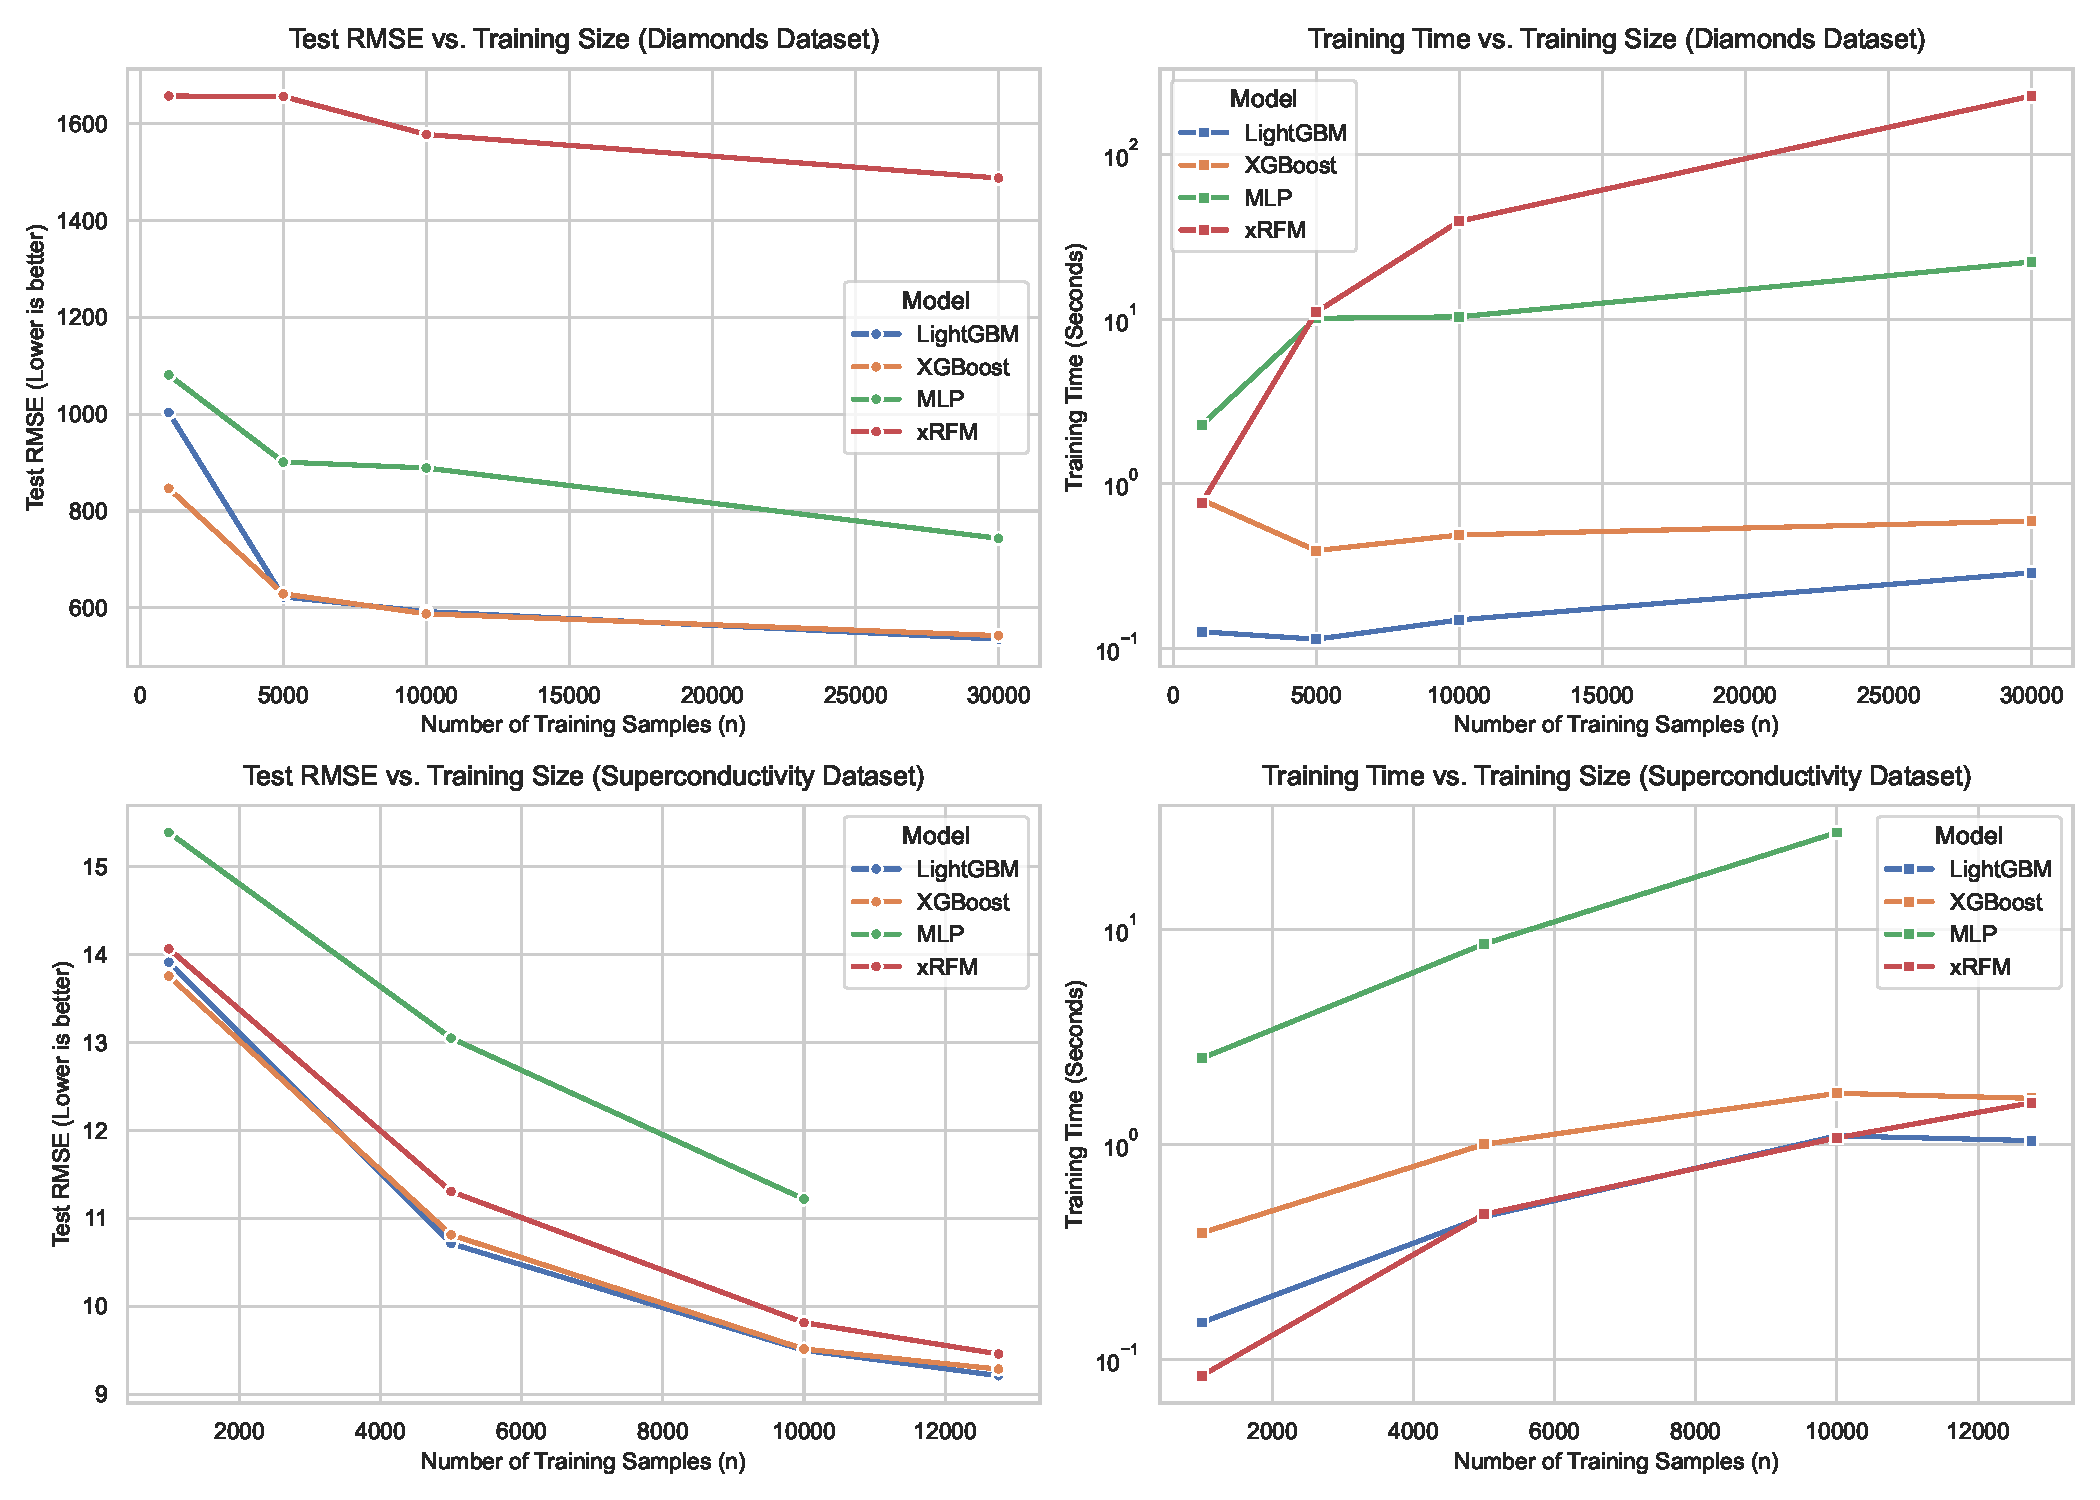
\includegraphics[width=\textwidth]{figures/scaling_analysis_2x2.pdf}
  \caption{Scalability analysis across Diamonds and Superconductivity datasets. The left column shows test RMSE, while the right column shows training time (in log-scale) as a function of training set size. This illustrates xRFM's steeper time complexity compared to the tree-based models.}
  \label{fig:scaling}
\end{figure}

On Diamonds, xRFM's training time grows from 0.77s to 226.44s as $n$ increases from 1{,}000 to 30{,}000, while its RMSE only improves from 1657.0 to 1487.5; LightGBM reaches 535.3 in under one second. On Superconductivity, xRFM scales more favourably, improving from 14.07 to 9.46 RMSE over the same range. As shown in Figure~\ref{fig:tradeoff}, the Pareto front analysis confirms that while xRFM approaches the performance of LightGBM on numerical datasets, it requires exponentially more training time.

\begin{figure}[htbp]
  \centering
  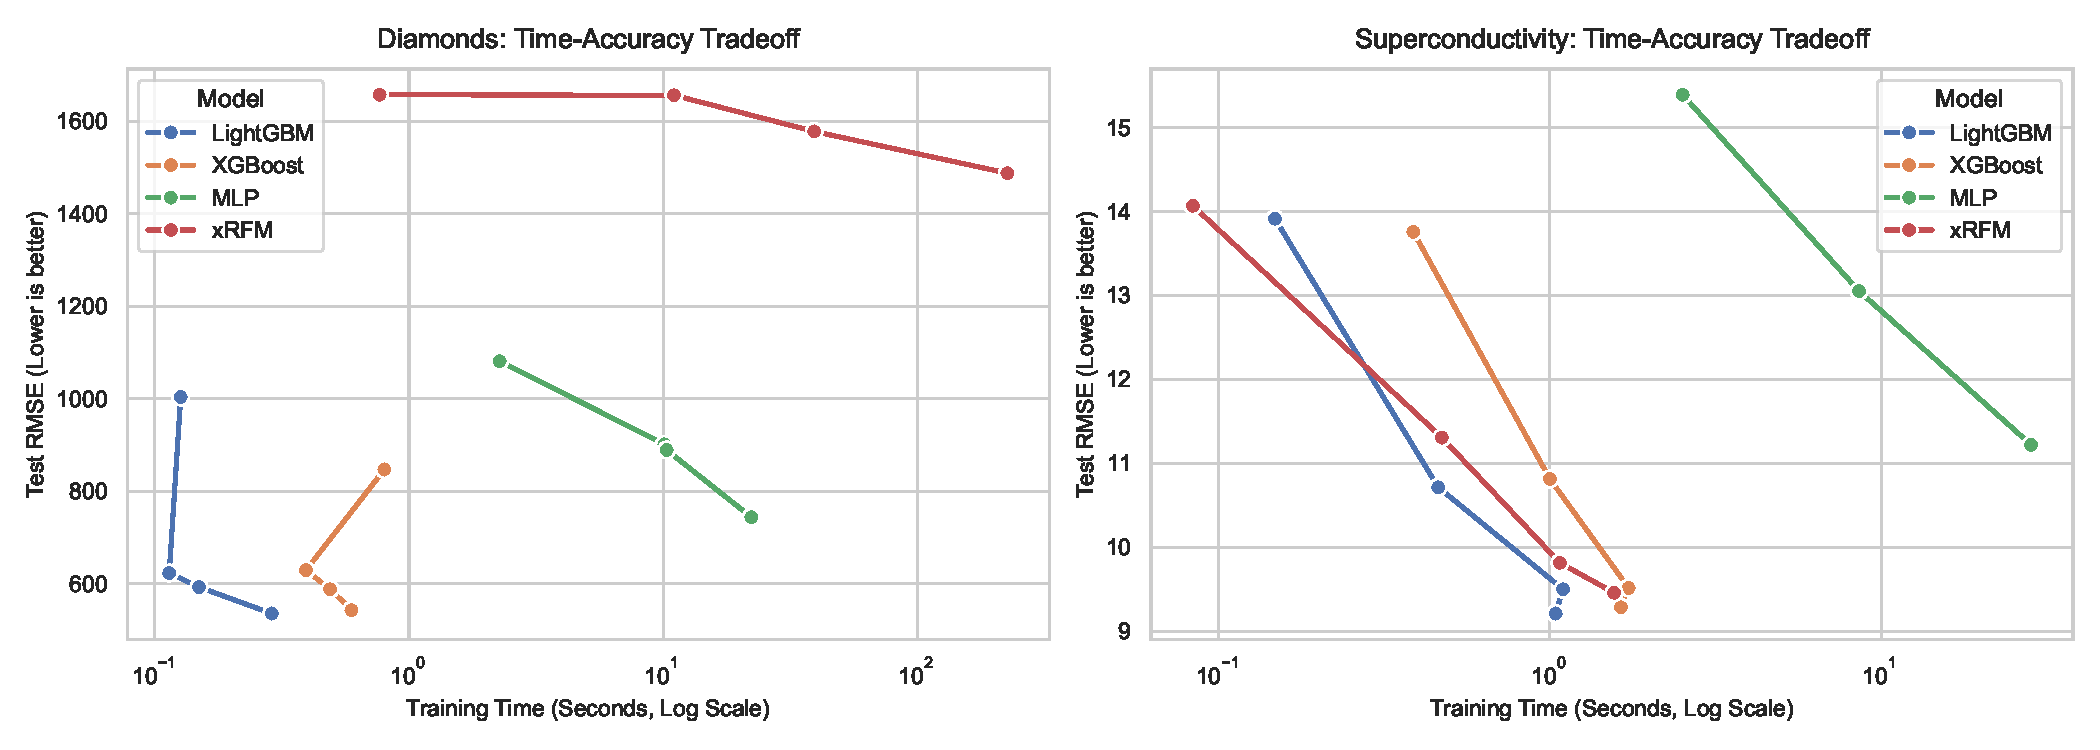
\includegraphics[width=\textwidth]{figures/time_accuracy_tradeoff.pdf}
  \caption{Time-Accuracy tradeoff comparison. The points for each model represent different training sizes ($n$). This visualization highlights the efficiency gap between AGOP reweighting and gradient boosting.}
  \label{fig:tradeoff}
\end{figure}

\subsection{Interpretability Comparison}

Figure~\ref{fig:feature-importance} visualises the top-five AGOP-ranked features extracted from the trained xRFM models for representative datasets.

\begin{figure}[htbp]
  \centering
  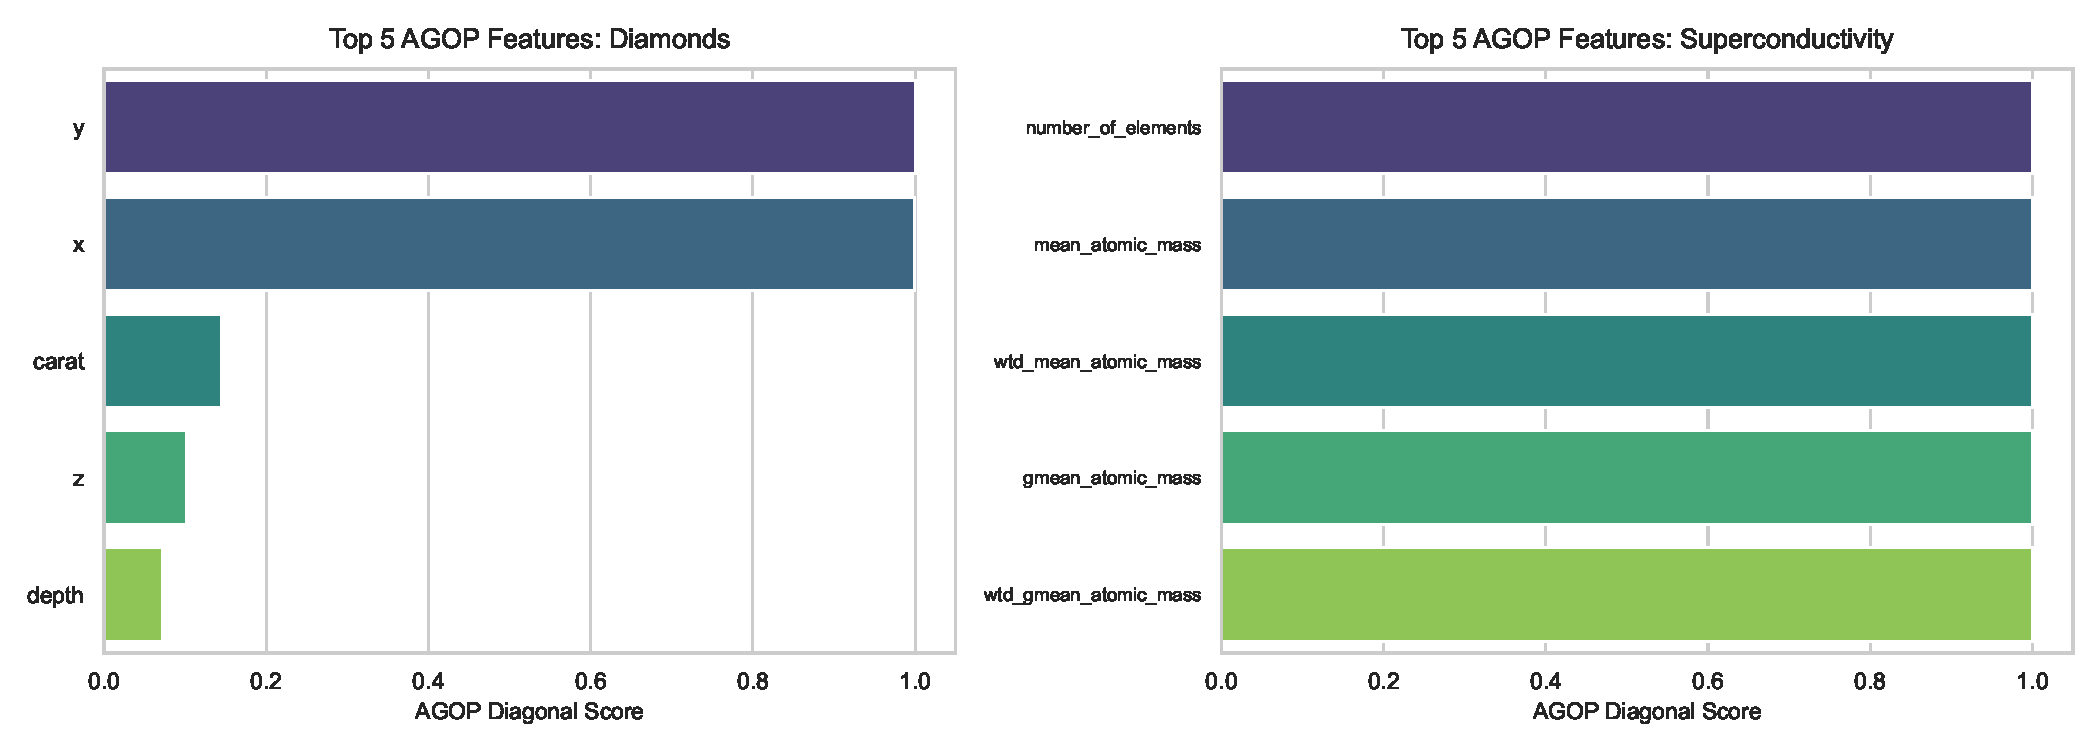
\includegraphics[width=\textwidth]{figures/feature_importance_bars.pdf}
  \caption{Top 5 feature importance rankings derived from the xRFM AGOP diagonal values for the Diamonds and Superconductivity datasets.}
  \label{fig:feature-importance}
\end{figure}

The AGOP rankings are broadly interpretable: physical size variables ($x, y, z$) for Diamonds and atomic mass variables for Superconductivity all align with domain knowledge[cite: 122]. Notably, the dominance of \texttt{y} and \texttt{x} in Diamonds reflects the learned function's high sensitivity to these continuous dimensions, despite the model's overall predictive lag behind GBDTs.

Table~\ref{tab:interpretability-methods} compares AGOP diagonal importance with PCA, mutual information, and permutation importance. These methods answer different questions.

\begin{table}[htbp]
  \centering
  \caption{Conceptual comparison of interpretability methods for tabular features.}
  \label{tab:interpretability-methods}
  \small
  \begin{tabular}{llll}
    \toprule
    Method & Supervised? & Model-specific? & Main interpretation \\
    \midrule
    AGOP diagonal          & Yes & Yes            & Sensitivity of xRFM to each feature \\
    PCA loadings           & No  & No             & Directions of maximum input variance \\
    Mutual information     & Yes & No             & Feature-target dependence \\
    Permutation importance & Yes & Model-agnostic & Performance drop after feature shuffle \\
    \bottomrule
  \end{tabular}
\end{table}

Notably, meaningful AGOP rankings do not imply strong predictive performance: on Diamonds, AGOP identifies sensible size-related features, yet xRFM's RMSE is nearly three times higher than LightGBM's[cite: 128]. This suggests that boosted trees capture axis-aligned thresholds more efficiently than AGOP reweighting, and that interpretability and accuracy can be decoupled[cite: 129].

% Section 4: Discussion

\section{Discussion}

\subsection{xRFM: When Feature Learning Helps and When It Does Not}

The empirical results partially support the motivation behind xRFM. The AGOP mechanism is designed to learn task-relevant feature directions rather than relying only on the original coordinate system~\citep{beaglehole2025xrfm,radhakrishnan2024mechanism}. This is most visible in the HR Attrition dataset, where xRFM achieves the highest accuracy among the four models. Since HR Attrition has only 882 training examples after splitting, this result suggests that xRFM can be competitive in small-data settings where a structured feature-learning prior may help stabilise prediction. The feature-importance ranking for this dataset is also plausible: overtime, business travel, and total working years are all work-condition variables that can reasonably relate to attrition.

However, the results also show clear limitations. The strongest negative case is Diamonds, where xRFM obtains 1496.72 RMSE, compared with 544.68 for XGBoost and 535.99 for LightGBM. This is not a small gap: xRFM is almost three times worse than the best tree-based model on this dataset. A likely algorithm-design explanation is that Diamonds contains strong axis-aligned effects and threshold-like categorical structure, such as cut, colour, clarity, and size variables. Boosted decision trees are highly effective at capturing such split-based interactions~\citep{friedman2001greedy,breiman2001random,chen2016xgboost,ke2017lightgbm}. By contrast, xRFM estimates task-relevant feature geometry through gradients and kernel-style feature learning. This can be less efficient when the dominant predictive structure is already well represented by simple tree splits.

The scalability experiment strengthens this interpretation. On Diamonds, xRFM improves only modestly as $n_\text{train}$ increases from 1{,}000 to 30{,}000, while its training time increases from less than one second to more than 226 seconds. This indicates that simply adding more data does not solve the inductive-bias mismatch for this dataset. In contrast, on Superconductivity, xRFM improves from 14.07 RMSE at 1{,}000 examples to 9.46 RMSE at the full training size, approaching the boosted-tree baselines. This dataset is fully numerical and high-dimensional, which may better match AGOP's objective of identifying useful continuous directions in feature space.

Therefore, xRFM appears most promising when the data are numerical or moderately high-dimensional, and when interpretability through learned feature sensitivity is important. It is less attractive when the task is large-scale mixed-type tabular regression with strong categorical threshold effects, where XGBoost and LightGBM remain more accurate and substantially more efficient~\citep{grinsztajn2022tree,holzmuller2024better}. Future improvements should focus on dataset-specific hyperparameter tuning, better handling of categorical variables, more efficient AGOP approximation, and integration with tree-style partitioning mechanisms.

\subsection{XGBoost and LightGBM: Performance and Efficiency}
\label{sec:gbdt-discussion}

XGBoost and LightGBM deliver competitive or superior performance across all five datasets while remaining the fastest models to train. On Diamonds, both GBDTs outperform xRFM by a large margin in RMSE (544.68 and 535.99 versus 1496.72), consistent with the strong axis-aligned inductive bias of tree-based splits~\citep{grinsztajn2022tree}. On HR Attrition ($n=882$, $d=51$), xRFM marginally surpasses XGBoost in accuracy (0.8673 versus 0.8571), suggesting that kernel-style feature learning offers a modest advantage only in a restricted small-data regime. LightGBM is the fastest model at every large Diamonds scale, with near-linear growth in training time (Table~\ref{tab:scaling}).

\subsection{MLP: Performance and Scalability Limitations}
\label{sec:mlp-discussion}

On Diamonds, MLP underperforms both XGBoost and LightGBM by a large margin in RMSE (743.5 versus 542.7 and 535.3 at $n=30{,}000$), and a similar pattern is observed on Superconductivity (11.22 versus approximately 9.5 RMSE) (Table~\ref{tab:main-results}), indicating weaker ability to exploit feature interactions without extensive architecture tuning~\citep{tolstikhin2021mlp,holzmuller2024better}. In classification tasks, performance is unstable: while accuracy can be comparable in some cases, such as Stroke, probability ranking degrades significantly, as reflected by the low AUC of 0.269 on Stroke. This highlights sensitivity to class imbalance and calibration issues~\citep{walde2004statistical}. Unlike tree-based methods, MLPs rely on global gradient-based optimisation over continuous parameter spaces. This makes them less aligned with the piecewise and often sparse structure of tabular features, resulting in lower data efficiency.

% ── Section 5: Conclusion ─────────────────────────────────────────────────────
% Responsible: E (with framework from overall report)

\section{Conclusion}

\textit{[Placeholder: Conclusion to be written by E ($\sim$0.25--0.5 page). Summarise: key findings, overall assessment of xRFM vs.\ baselines, future directions.]}


% ── Appendix ──────────────────────────────────────────────────────────────────
\newpage
\phantomsection
\addcontentsline{toc}{section}{Appendix}
\appendix
% ── Appendix: Bonus ───────────────────────────────────────────────────────────

\section{AGOP-Based Splitting Criterion: Scratch Implementation}
\label{app:bonus}

The xRFM tree selects the split direction at each node as the leading
eigenvector $v_1$ of the AGOP $G_f = \mathbb{E}_x[\nabla f(x)\nabla
f(x)^\top]$~\citep{beaglehole2025xrfm}.  We implement this criterion from
scratch using Ridge regression ($f(x)=w^\top x+b$, $\alpha=10^{-3}$).  For a
linear model the gradient is constant so the AGOP simplifies to
$G_f = ww^\top$, giving the closed-form diagonal $[G_f]_{ii}=w_i^2$ and split
direction $v_1 = w/\|w\|$.  The optimal threshold $t^*$ is found by scanning
30 candidate quantiles of $v_1^\top X$ and picking the one that minimises
weighted target variance.  The full implementation is in
\texttt{bonus/agop\_split.py}.

\paragraph{Verification.}
We use a synthetic dataset ($n=300$, $d=10$) with $y=3x_0-2x_1+\varepsilon$,
so the ground-truth signal features are $\{x_0,\,x_1\}$.  We compare the
scratch AGOP diagonal $w_i^2$ against a numerical AGOP diagonal computed by
finite-difference gradients of the fitted xRFM predictor (black-box use only).

\begin{table}[H]
  \centering
  \caption{AGOP diagonal on the synthetic dataset. Noise features $x_2$–$x_9$
           score $\le 0.03$ (scratch) and $\le 0.30$ (xRFM).}
  \label{tab:bonus-agop}
  \small
  \begin{tabular}{lcc}
    \toprule
    Feature & Scratch $w_i^2$ & xRFM numerical \\
    \midrule
    $x_0$ (coef.\ $+3$) & 9.23 & 13.03 \\
    $x_1$ (coef.\ $-2$) & 3.93 &  5.28 \\
    $x_2$–$x_9$ (noise) & $\le 0.03$ & $\le 0.30$ \\
    \midrule
    Top-2 identified & $\{x_0,x_1\}$ & $\{x_0,x_1\}$ \\
    Cosine similarity & \multicolumn{2}{c}{\textbf{0.9985}} \\
    \bottomrule
  \end{tabular}
\end{table}

Both methods identify $\{x_0,x_1\}$ correctly (overlap 2/2, cosine similarity
0.9985), confirming that the scratch criterion recovers the same split direction
as the xRFM library.


% ── References ────────────────────────────────────────────────────────────────
\newpage
\phantomsection
\addcontentsline{toc}{section}{References}
\bibliographystyle{plainnat}
\bibliography{sections/references}

\end{document}
